% Laborationsmall.tex
\documentclass[a4paper]{article}

\usepackage[swedish]{babel}
\usepackage[utf8x]{inputenc}

\usepackage{multicol}
\usepackage[vmargin=3cm,hmargin=2cm]{geometry}
\usepackage{parskip}
\usepackage[runin]{abstract}
\renewcommand{\abstitleskip}{0mm}

\usepackage{hyperref}
\usepackage{amsmath}
\usepackage{lmodern}
\usepackage[T1]{fontenc}
\usepackage{tikz}
\usetikzlibrary{decorations.pathreplacing}
\usetikzlibrary{arrows.meta}

\addto\extrasswedish{%
	\def\equationautorefname{Ekvation}%
	\def\figureautorefname{Figur}%
	\def\tableautorefname{Tabell}%
	\def\sectionautorefname{Rubrik}%
	\def\subsectionautorefname{Underrubrik}%
	\def\pageautorefname{Sida}%
}

\usepackage{graphicx}
\usepackage{ccaption}
\captionnamefont{\it}
\captiontitlefont{\it}

% Hack för att få komma istället för punkt i matematiska uttryck
% $3.141592$ blir 3,141592
% Om man använder komma direkt får man ett litet oönskat mellanrum:
% $3,141592$ blir 3, 141592
\DeclareMathSymbol{,}{\mathpunct}{letters}{"3B}
\DeclareMathSymbol{.}{\mathord}{letters}{"3B}
\DeclareMathSymbol{\decimal}{\mathord}{letters}{"3A}

% Kommando för att få icke-kursiva enheter i matematiska uttryck
% $10\unit{km}$ blir 10 km
\newcommand{\unit}[1]{\ensuremath{\,\mathrm{#1}}}

\usepackage{lastpage}
\usepackage{fancyhdr}
\pagestyle{fancy}
\fancyhf[C]{\thepage}
\fancyhead[C]{Våglära och optik, FAFF30}
\fancyhead[R,L]{}
\fancypagestyle{plain}{
  \fancyhead{}
}
\setcounter{secnumdepth}{-1}

\title{Laborationen ”Polarisation”}
\author{Johan Mauritsson\\Lunds Universitet}

\makeatletter
\renewcommand{\section}{\@startsection
{section}%                   % the name
{1}%                         % the level
{0mm}%                       % the indent
{-\baselineskip}%            % the before skip
{0.5mm}%          % the after skip
{\normalfont\bfseries}} % the style
%\renewcommand{\sectionmark}[1]{ }
%\renewcommand{\thesection}{}

\renewcommand*\maketitle{
  {
    \begin{center}
      {\huge\bfseries \@title}\\
      \vspace{5mm}
      {\large \@author}
    \end{center}
    \vspace{2mm}
  }
}
\makeatother

\begin{document}
\maketitle


\begin{abstract}
  Kort beskrivning  av resultaten (5-10  rader). Det ska inte  vara en
  innehållsbeskrivning (först gör vi det, sen använder vi den metoden,
  och så jämför vi det med de där tidigare kända resultaten, etc) utan
  vara   koncentrerat  till   ”resultatet”,   vad   man  kommer   fram
  till. Sammanfattningen är uppsatsens löpsedel. Den ska vara kort och
  kärnfull och locka läsare genom att  effektivt göra klart vad det är
  man uppnår genom att läsa rapporten.
\end{abstract}

\vspace{2mm}

\hspace{-3mm}
\begin{tabular}{ll}
Laborationen genomförd: &	2017-03-27 \\
Rapporten kamratgranskad: &	2013-xx-xx \\
Lämnad till handledare: &	2013-xx-xx \\
\end{tabular}

\vspace{3mm}

\begin{multicols}{2}
  \section*{Inledning}
  %Preliminär beskrivning av uppgiften  i lättfattliga termer. Bakgrunden till att man intresserar sig för detta problem, denna uppgift. Hur den ingår i ett större sammanhang.

%  En detaljerad beskrivning av vad det hela går ut på, och vad exakt din uppgift   i    sammanhanget   är.    Utrustningsförutsättningar.   Det
%  ursprungligen avsedda målet. Även den i ämnet oinsatte ska ha en ärlig
%  chans att förstå de stora dragen.
%
%  Beskrivning av hur rapporten är uppbyggd, för att göra det möjligt för
%  läsaren att förstå vad som  pågår, ge läsaren rätta förväntningar, och
%  för  att  underlätta direktåtkomst  av  för  den individuelle  läsaren
%  särskilt intressanta delar.

  \section{Teori}
  
  

  \begin{align} 
  \label{eq:alphaPrim}
  \alpha' &= \arcsin\left(\frac{\sin\alpha}{n}\right)\\
  \label{eq:beta}
  \beta &= \arcsin\left(n \sin\beta'\right)\\
  \label{eq:betaPrim}
  \beta' &= A-\alpha'\\
  \label{eq:delta}
  \delta &= \alpha+\beta-\alpha'-\beta'
  \end{align}

  \begin{equation} \label{eq:avlänkning}
  \delta = \alpha-A+\arcsin\left(n \sin\left(A-\arcsin\left(\frac{\sin\alpha}{n}\right)\right)\right)
  \end{equation}

  \section{Metod}
  % De  olika  stegen  i  uppgiftens genomförande.  Till  exempel  val  av
  % algoritmer,  programspråk och  annan programvara,  undersökningsmetod,
  % statistiska  metoder. Där  valmöjligheter finns,  diskutera de  gjorda
  % valen.
  
  % Beskrivning av mätning av fokallängd här.
  
  En laser leddes genom ett optiskt fiber och en lins användes för att kollimera stålen när den lämnade fibret. Två irisar placerades på en väldefinierad linje och lasern leddes genom dessa för att bekräfta att lasern var rak och kollimerad.
  
  Ett prisma på en graderad roterbar platta placerades i laserstrålens väg och en millimetergraderad skärm placerades ut parallell med laserstrålen så att den brutna strålen träffade skärmen enligt \autoref{fig:exp}. Prismat roterades så att laserstrålen träffade rakt på ($\alpha=0$) och prismats rotation antecknades. Sedan roterades prismat 2\textdegree upprepade gånger och positionen där laserstrålen träffade skärmen antecknades och räknades om till vinkeln $\gamma$.
  
  Mätvärdena matades in i matlab och där användes appen ``Curve Fitting'' för att hitta ett brytningsindex så att ekvationen \eqref{eq:avlänkning} gäller så väl som möjligt.

  \section{Resultat}
  %Vad man  kommer fram till?  Om uppgiften innebär programmering  så kan
  %det färdiga programmet i sig vara resultatet.  Här är det i så fall på
  %sin  plats  med  beskrivningar  av programmet,  till  exempel  teknisk
  %beskrivning,    funktionell    beskrivning,    användningsbeskrivning,
  %användargränssnitt  etc.  Genomförandebeskrivning  kommer  i  så  fall
  %närmast att handla om programutvecklingen.

  %Men det kan också vara så  att det snarare är programmets beteende som
  %är resultatet.  Man utvecklar till  exempel en numerisk metod  för att
  %lösa ett problem,  och sedan gör man experiment  med testkörningar och
  %analyserar dessa test.

  \section{Diskussion}
  %Är resultaten rimliga? Vad hade kunnat göras annorlunda?

  \section{Slutsats/avslutning}
  %En   sammanfattning  där   man  till   skillnad  från   den  inledande
  %sammanfattningen förutsätter  att läsaren har läst  rapporten, samt de
  %slutsatser man kan dra av det gjorda arbetet.

  \section{Referenser}
  %Den använda litteraturen.

  \section{Appendix}
  %Eventuell     användarhandledning,     källkod,    anvisningar     för
  %systemgenerering, och liknande som inte  är av omedelbart intresse för
  %den ordinäre läsaren, läggs lämpligen som appendix.

\end{multicols}

\begin{figure}[h]
	\centering
	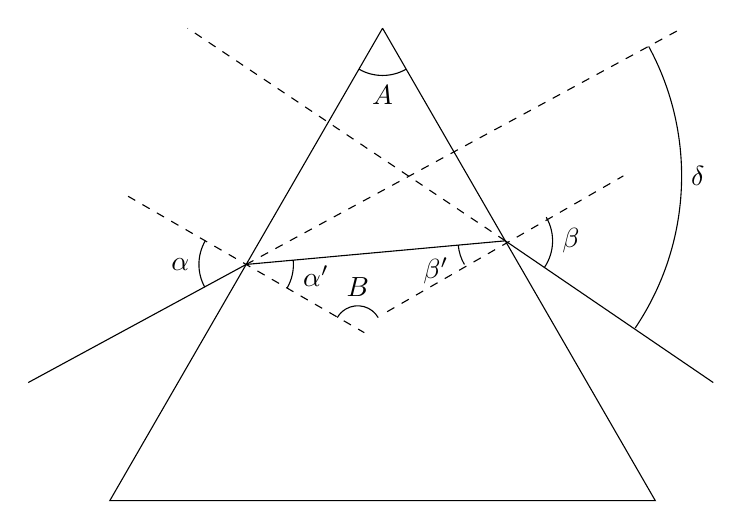
\begin{tikzpicture}[scale=1.5]
		\draw (0, 0) -- ({4/sqrt(3)}, -4) -- ({-4/sqrt(3)}, -4) -- (0, 0); % Triangeln
		
		\draw (-3, -3) -- ({-2/sqrt(3)}, -2) -- ({1.8/sqrt(3)}, -1.8) -- (2.8, -3); % Den brutna ljusstrålen
		\draw [dashed] ({-2/sqrt(3)}, -2) -- ({6 - 2*sqrt(3)}, 0); % Hjälplinjer
		\draw [dashed] ({1.8/sqrt(3)}, -1.8) -- (-1.65, 0);
		\draw [dashed] ({-2/sqrt(3)-1}, {-(6-sqrt(3))/3}) -- ({-2/sqrt(3)+1}, {-(6+sqrt(3))/3});
		\draw [dashed] ({1.8/sqrt(3)-1}, -2.4) -- ({1.8/sqrt(3)+1}, -1.25);
		
		\draw ({-0.4/2}, {-0.4*sqrt(3)/2}) arc [radius=0.4, start angle=240, end angle=300]; % Toppvinkeln
		\draw ({-2/sqrt(3) - (sqrt(3)*0.4)/2}, {-2 + 0.4/2}) arc [radius=0.4, start angle=150, end angle={150+58.45}]; % Infallsvinkeln
		\draw ({0.23 + 2.3*0.83}, {-1.25 - 2.3*0.56}) arc [radius=2.3, start angle=-34, end angle=28.5]; % Avlänkningsvinkeln
		\draw ({1.8/sqrt(3) + 0.4*0.83}, {-1.8 - 0.4*0.56}) arc [radius=0.4, start angle=-34, end angle=30]; % Lämningsvinkeln
		\draw ({-2/sqrt(3) + 0.4*sqrt(3)/2}, {-2 - 0.4*0.5}) arc [radius=0.4, start angle=-30, end angle=5.2]; % Hjälpvinklar
		\draw ({1.8/sqrt(3) - 0.4*0.996}, {-1.8 - 0.4*0.091}) arc [radius=0.4, start angle=185.2, end angle=210];
		\draw ({-0.21 + 0.2*sqrt(3)/2}, {-2.55 + 0.2*0.5}) arc [radius=0.2, start angle=30, end angle=150];
		
		\node [left] at ({-2/sqrt(3)-0.4}, -2) {$\alpha$};
		\node [right] at ({-2/sqrt(3)+0.4}, -2.1) {$\alpha'$};
		\node [left] at ({1.8/sqrt(3)-0.4}, -2.05) {$\beta'$};
		\node [right] at ({1.8/sqrt(3)+0.4}, -1.8) {$\beta$};
		\node [right] at ({0.23 + 2.3}, -1.25) {$\delta$};
		\node [below] at (0, -0.4) {$A$};
		\node [above] at (-0.21, -2.35) {$B$};
	\end{tikzpicture}
	\caption{Ljusstråle som bryts genom ett prisma med de hjälpvinklar som behövs för att räkna ut avlänkningsvinkeln.}
	\label{fig:prisma}
\end{figure}
\begin{figure}[h]
	\centering
	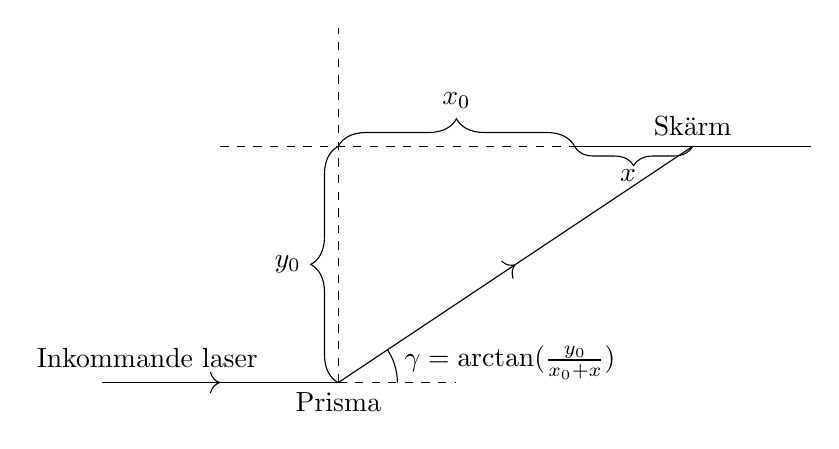
\begin{tikzpicture}[scale=1.5]
		\draw [decorate,decoration={brace,amplitude=10pt}] (0, 0) -- (0, 2) node [midway,left,xshift=-10pt] {$y_0$};
		\draw [decorate,decoration={brace,amplitude=10pt}] (0, 2) -- (2, 2) node [midway,above,yshift=10pt] {$x_0$};
		\draw [decorate,decoration={brace,amplitude=7pt,mirror}] (2, 2) -- (3, 2) node [midway,below,yshift=-5pt,xshift=-2pt] {$x$};
		\draw [dashed] (0, 0) -- (0, 3);
		\draw [dashed] (-1, 2) -- (2, 2);
		\draw (2, 2) -- (4, 2);
		\draw [-{>[scale=1.5]}] (0, 0) -- (1.5, 1);
		\draw (1.5, 1) -- (3, 2);
		\node [below] at (0, 0) {Prisma};
		\node [above] at (3, 2) {Skärm};
		\draw (0.5, 0) arc [radius=0.5, start angle=0, end angle={atan(2/3)}] node [midway,right,yshift=1pt] {$\gamma=\arctan(\frac{y_0}{x_0+x})$};
		\draw [-{>[scale=1.5]}] (-2, 0) -- (-1, 0) node [midway,above,xshift=-5pt,yshift=2pt] {Inkommande laser};
		\draw (-1, 0) -- (0, 0);
		\draw [dashed] (0, 0) -- (1, 0);
	\end{tikzpicture}
	\caption{Experimentuppställning}
	\label{fig:exp}
\end{figure}

\section{\LaTeX-kommentarer}
Kompileras enklast med \texttt{pdflatex}. Använd TeX Live i Linux och
MiKTeX i Windows.

Test av ”komma-hack” och enhetskommando (se källkod):
\hrule
\begin{minipage}{0.5\linewidth}
  Kod
\begin{verbatim}
\[ \Delta x = 1.23\unit{km} \]
\end{verbatim}
\end{minipage}
\begin{minipage}{0.5\linewidth}
  Resultat\\
  $ \Delta x = 1.23\unit{km} $
\end{minipage}

\end{document}
